\chapter{Workpiece Data Programming}

\section{Manual Data Entry Without Memory (TEACH IN/MDI)}

\procedure

\begin{itemize}
    \iconitem {Press the \textbf{TEACH IN} button.}{teach_in.jpg}
\end{itemize}

The following display appears on the screen:

\begin{figure}[h]
    \centering
    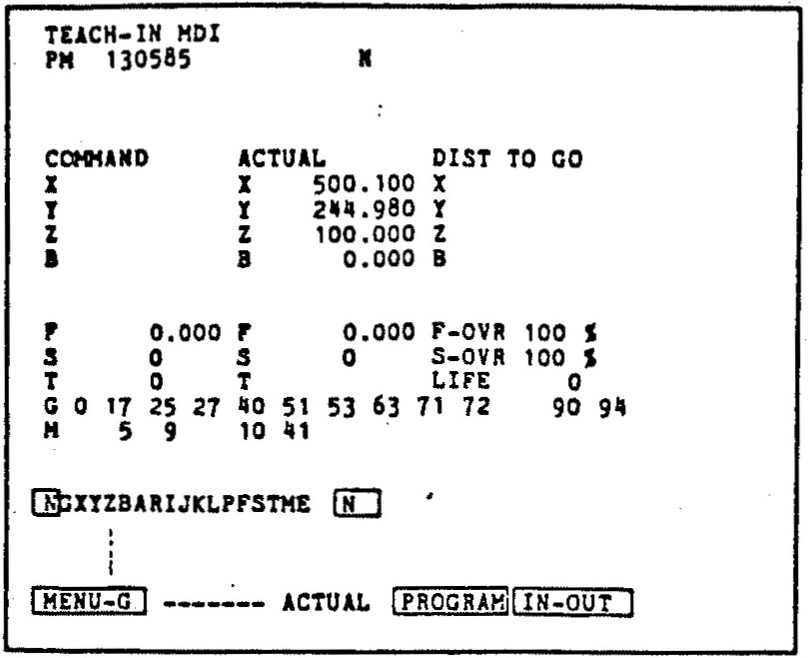
\includegraphics[width=0.7\textwidth]{teach_in_screen.jpg}
    \caption{TEACH IN/MDI Mode Display}
\end{figure}

\begin{itemize}
    \iconitem {Move the cursor to the corresponding address letter using the \textbf{left} and \textbf{right} command buttons.}{left.jpg, right.jpg}
\end{itemize}

\vspace{.5cm}

\begin{itemize}
    \item Enter the numerical value using the keyboard.
\end{itemize}

\begin{itemize}
    \iconitem {Press the \textbf{ENTER} button for each program word consisting of an address letter and a numerical value.}{enter.jpg}
\end{itemize}

\vspace{.5cm}

\begin{itemize}
    \iconitem {Press the \textbf{START} button after entering all program words for a block.}{start.jpg}
\end{itemize}

Pressing the \textbf{START} button executes all instructions entered in the program block.

\begin{itemize}
    \iconitem {Press the \textbf{MANUAL} button to deactivate \textbf{TEACH IN/MDI} mode.}{manual.jpg}
\end{itemize}

\newpage

\notes

\begin{itemize}
    \item The programmed feed rate in the block can be adjusted within a range of \textbf{0 to 140\%} using the feed rate adjustment buttons.
    \item The programmed \textbf{rapid feed rate} can only be modified within the range of \textbf{0 to 100\%}.
    \item The actual speed is displayed on the screen under \textbf{ACTUAL}.
    \item The cursor jumps from one address letter to the next if a \textbf{left} or \textbf{right} command button is held down for more than one second.
\end{itemize}

\textbf{Error message clearing:} See \textbf{Section 2.1}.

\textbf{Graphical interface and operator guidance:} See \textbf{Section 3}.

\section{Spindle Speed Adjustment (Spindle Potentiometer)}

\textbf{ONLY FOR MAIN MOTOR WITH ANALOG SPEED VARIATION!}

Spindle speed adjustments (affecting the main spindle) are only applicable for an analog control system.

The spindle speed can be modified within a range of \textbf{80 to 120\%}, in increments of \textbf{5\%}, relative to the programmed value. This applies to all operating modes.


\begin{itemize}
    \iconitem {Pressing the \textbf{-5\%} adjustment button decreases the spindle speed by \textbf{5\%} within the specified range.}{decrease_5.jpg}
\end{itemize}

\begin{itemize}
    \iconitem{Pressing the \textbf{+5\%} adjustment button increases the spindle speed by \textbf{5\%} within the specified range.}{increase_5.jpg}
\end{itemize}

\begin{itemize}
    \iconitem {Holding either adjustment button for more than one second continuously adjusts the spindle speed in \textbf{5\% increments} without interruption.}{hold_5.jpg}
\end{itemize}

\begin{itemize}
    \item The spindle speed can be reset to the programmed value by pressing the corresponding button.
\end{itemize}

If a new spindle speed is programmed, any previous manual adjustments are automatically overridden, and the spindle potentiometer is reset to \textbf{100\%}.

\marginnoteicon{17.7cm}{manual_spindle_adjustment.jpg}[0.4cm]

In \textbf{MANUAL mode}, the spindle speed can be reduced to its lowest value using the \textbf{jog feed rate control}, as long as the corresponding button is held down.

\newpage

\section{Manual Data Entry with Memory (TEACH IN/PLAYBACK)}

\procedure

\begin{itemize}
    \iconitem {Press the \textbf{TEACH IN} button.}{teach_in.jpg}
\end{itemize}

\vspace{.5cm}

\begin{itemize}
    \iconitem {Press the \textbf{MENU} button.}{menu.jpg}
\end{itemize}
\vspace{.5cm}
The following display appears on the screen:

\begin{figure}[h]
    \centering
    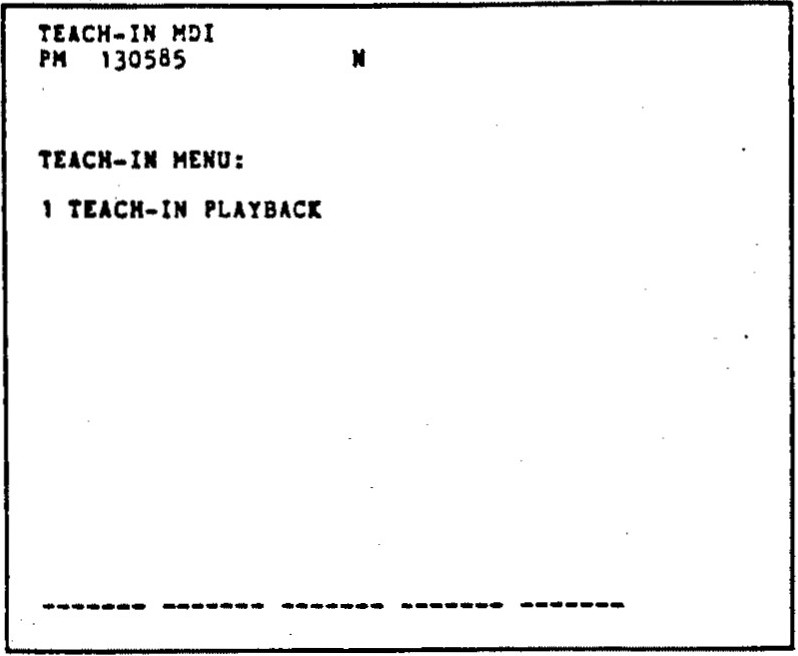
\includegraphics[width=0.6\textwidth]{teach_in_menu.jpg}
\end{figure}

\begin{itemize}
    \item Press key \textbf{1} on the numeric keypad to select \textbf{TEACH IN PLAYBACK}.
\end{itemize}

The following display appears on the screen:

\begin{figure}[h]
    \centering
    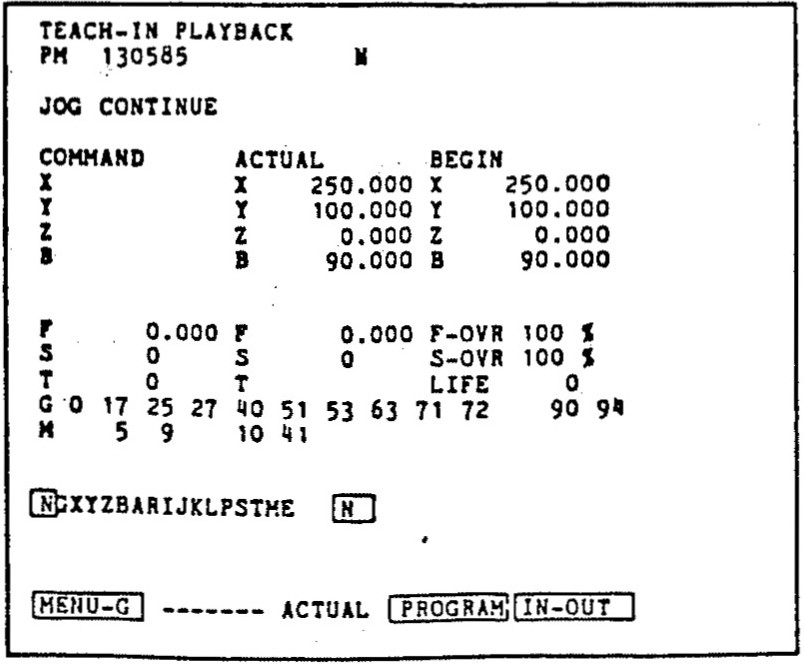
\includegraphics[width=0.6\textwidth]{teach_in_playback.jpg}
\end{figure}
\newpage
\begin{itemize}
    \iconitem{ Move the cursor to the address letter \textbf{N} using the \textbf{left} and \textbf{right} command buttons.}{left.jpg, right.jpg}
\end{itemize}

\vspace{.5cm}

\begin{itemize}
    \item Enter a program number using the numeric keypad.
\end{itemize}

\begin{itemize}
    \iconitem {Press the \textbf{ENTER} button.}{enter.jpg}
\end{itemize}

\vspace{.5cm}

\begin{itemize}
    \iconitem {Press the \textbf{STORE} button.}{store.jpg}
\end{itemize}

Pressing the \textbf{STORE} button saves the program number in memory, and the first program block \textbf{N1} appears on line 21 of the screen.

\subsection{TEACH IN Mode}

The operator guidance function, which greatly facilitates programming, is activated when using **manual data entry with memory**.

When the operator enters a \textbf{G function} (movement condition), only the required address letters for inputs conditioning the execution of that \textbf{G function} remain displayed on **line 5** of the screen.

\procedure

\begin{itemize}
    \iconitem {Move the cursor to the desired address letter using the \textbf{left} and \textbf{right} command buttons.}{left.jpg, right.jpg}
\end{itemize}

\vspace{.5cm}

\begin{itemize}
    \item Enter the numerical value using the keyboard.
\end{itemize}

\begin{itemize}
    \iconitem {Press the \textbf{ENTER} button after each program word entry (address letter + numerical value).}{enter.jpg}
\end{itemize}

\vspace{.5cm}

\begin{itemize}
    \iconitem {Press the \textbf{START} button after entering all program words for a block.}{start.jpg}
\end{itemize}

Pressing the \textbf{START} button executes all instructions entered in the program block.

If the program block executes correctly:

\begin{itemize}
    \iconitem {Press the \textbf{STORE} button.}{store.jpg}
\end{itemize}

\vspace{.5cm}

\begin{itemize}
    \iconitem {The \textbf{MANUAL} and \textbf{CLEAR CONTR.} buttons can be used to exit TEACH IN/PLAYBACK mode.}{manual.jpg,clear_contr.jpg}
\end{itemize}

\newpage

\notes

\begin{itemize}
    \item The current block can be modified and executed again as long as the \textbf{STORE} button has not been pressed.
    \item Pressing the \textbf{STORE} button saves the entire block in memory, and the number of the next block appears on \textbf{line 21} of the screen.
    \item Program blocks saved in memory can no longer be modified in **TEACH IN/PLAYBACK mode**.
\end{itemize}

\textbf{Graphical interface and operator guidance:} See Section 3.

\textbf{Modifications, insertions, and deletions of program words:} See Section 6.2.2.

\textbf{Deleting a program block:} See Section 6.2.3.

It is possible to \textbf{insert additional blocks} into the program later in **TEACH IN/PLAYBACK mode**.

\procedure

\begin{itemize}
    \iconitem {Move the cursor to the address letter \textbf{N} using the \textbf{left} and \textbf{right} command buttons.}{left.jpg,right.jpg}
\end{itemize}

\vspace{.5cm}

\begin{itemize}
    \item Enter the block number \textbf{before} which the new block should be inserted.
\end{itemize}

\begin{itemize}
    \iconitem {Press the \textbf{ENTER} button.}{enter.jpg}
\end{itemize}

\vspace{.5cm}

\begin{itemize}
    \iconitem {Press the \textbf{SEARCH} button.}{search.jpg}
\end{itemize}

\vspace{.5cm}

\begin{itemize}
    \iconitem {Move the cursor back to the address letter \textbf{N} using the \textbf{left} and \textbf{right} command buttons.}{left.jpg, right.jpg}
\end{itemize}

\vspace{.5cm}

\begin{itemize}
    \item Enter the number of the block that should be inserted (**this number must not yet exist in the program**).
\end{itemize}

\begin{itemize}
    \iconitem {Press the \textbf{ENTER} button.}{enter.jpg}
\end{itemize}

\vspace{.5cm}

The block to be inserted can now be entered by following the previously described procedure.

\newpage

\subsubsection*{End of Program Block Handling}

If the final program block does not include the word \textbf{M30}, press the \textbf{STORE} button immediately after pressing \textbf{ENTER} (without pressing the \textbf{START} button).

The functions \textbf{G41} and \textbf{G42} should not be used in \textbf{TEACH IN/PLAYBACK mode}.

The function \textbf{G22} can be used.

\textbf{Error Message Clearing:} See \textbf{Section 2.1}.

If it becomes necessary to exit \textbf{TEACH IN/PLAYBACK mode} by pressing the \textbf{MANUAL} and \textbf{CLEAR CONTR.} buttons, the system must be switched back to \textbf{TEACH IN/PLAYBACK mode} after resolving the issue (see \textbf{Section 3.3.3}).

\subsection{PLAYBACK Mode}

Positions on the workpiece are not entered via the keyboard but are instead referenced in step mode.

During step-mode positioning, the \textbf{adjusted feed rate} (modified using the feed rate override buttons) is active and displayed on the screen under \textbf{ACTUAL}.

\textbf{The last F word} of the currently stored program block is used for that block \textbf{unless a new F word has been written into the block before storing}.

If the current program block does not contain an \textbf{F word}, for example, when executing step movements immediately after entering a program number, the fixed feed rate stored in the \textbf{machine constants} is used. In this case:

\begin{itemize}
    \item The step feed rate \textbf{is not adjusted} using the feed rate override buttons.
    \item The feed rate display on the screen under \textbf{ACTUAL} is active and automatically applied in the next block if it contains an \textbf{F word}.
    \item However, the \textbf{F word remains ineffective for a block entered in TEACH IN mode}.
\end{itemize}

All other \textbf{program words} must be written into the block according to the previously described \textbf{procedure} before they are stored.

\newpage

\subsubsection*{Positioning and Mode Switching}

All positions must be referenced within a program block, either in \textbf{step mode (PLAYBACK)} or entered via the keyboard in \textbf{TEACH IN} mode. However, it is possible to switch freely between program modes from one block to another.

\procedure

\begin{itemize}
    \iconitem {Press the feed rate override buttons.}{decrease_5.jpg, increase_5.jpg}
    \vspace{.5cm}
    \item Reference the positions on the workpiece by pressing the corresponding axis movement buttons.
    \item The feed rate can be adjusted freely within a range of \textbf{0 to 140\%} using the respective override buttons.
\end{itemize}

Additionally, \textbf{incremental step movement} mode can be used for axis positioning (see \textbf{Section 2.2.2}).

\begin{itemize}
    \item If necessary, enter other program words into the block (see \textbf{Section 3.3.1}), e.g., the feed rate value at address \textbf{F}, which will be activated later in the block when the program executes.
\end{itemize}

\begin{itemize}
    \iconitem {Press the \textbf{STORE} button.}{store.jpg}
\end{itemize}

\vspace{.5cm}

\begin{itemize}
    \iconitem {Exit \textbf{TEACH IN/PLAYBACK} mode by pressing the \textbf{MANUAL} and \textbf{CLEAR CONTR.} buttons.}{manual.jpg, clear_contr.jpg}
\end{itemize}
\vspace{.5cm}
\notes

\begin{itemize}
    \item It is possible to correct positions on the workpiece in step mode, as well as modify program block words, as long as the \textbf{STORE} button has not been pressed.
    \item After any modification, the block must be executed again by pressing the \textbf{START} button before pressing \textbf{STORE} to save it.
\end{itemize}

See also the remarks at the end of \textbf{Section 3.3.1}.

\newpage

\subsection{Resuming TEACH IN/PLAYBACK Mode}

Follow this procedure to return to \textbf{TEACH IN/PLAYBACK} mode if programming was interrupted by pressing the \textbf{MANUAL} and \textbf{CLEAR CONTR.} buttons.

\begin{itemize}
    \iconitem {Press the \textbf{TEACH IN} button.}{teach_in.jpg}
    \vspace{.6cm}
    \iconitem {Press the \textbf{MENU} button.}{menu.jpg}
    \vspace{.6cm}
    \item Press the numeric key \textbf{1} to select \textbf{TEACH IN PLAYBACK} mode.
\end{itemize}

\begin{itemize}
    \iconitem {Press the button labeled \textbf{Softkey F4}.}{f4.jpg}
    \vspace{.6cm}
    \item Enter any block number using the numeric keypad. The entered number must be \textbf{higher} than the last saved block.
    \iconitem {Press the \textbf{ENTER} button.}{enter.jpg}
    \vspace{.6cm}
    \iconitem {Press the \textbf{SEARCH} button.}{search.jpg}
\end{itemize}

\vspace{.5cm}
The last saved block in \textbf{TEACH IN/PLAYBACK} mode is automatically retrieved and displayed on the screen.

The resumption procedure is complete after entering the \textbf{next block number} and pressing the \textbf{Softkey F4} button. Programming can now continue.

\newpage

\section{Workpiece Origin Determination}

The workpiece origin is referenced to the workpiece itself, while the machine origin is referenced to the machine.

Both reference points must be defined relative to each other for correct machining program execution. This is achieved by setting the workpiece origin relative to the machine axes.

\subsection{Setting the Workpiece Origin on Machine Axes (RESET AXIS)}

\begin{itemize}
    \item Reference the machine axes (see Section 2.5).
    \item Reference the workpiece origin step by step (see Section 2.2).
    \item Read and record the actual values for the machine axes displayed under \textbf{ACTUAL}.
\end{itemize}

The recorded values define the \textbf{offset between the workpiece origin and the machine origin}.


\begin{itemize}
    \iconitem {Press the \textbf{MENU} button.}{menu.jpg}
\end{itemize}

The main menu of the command sub-modes appears on the screen:

\begin{figure}[h]
    \centering
    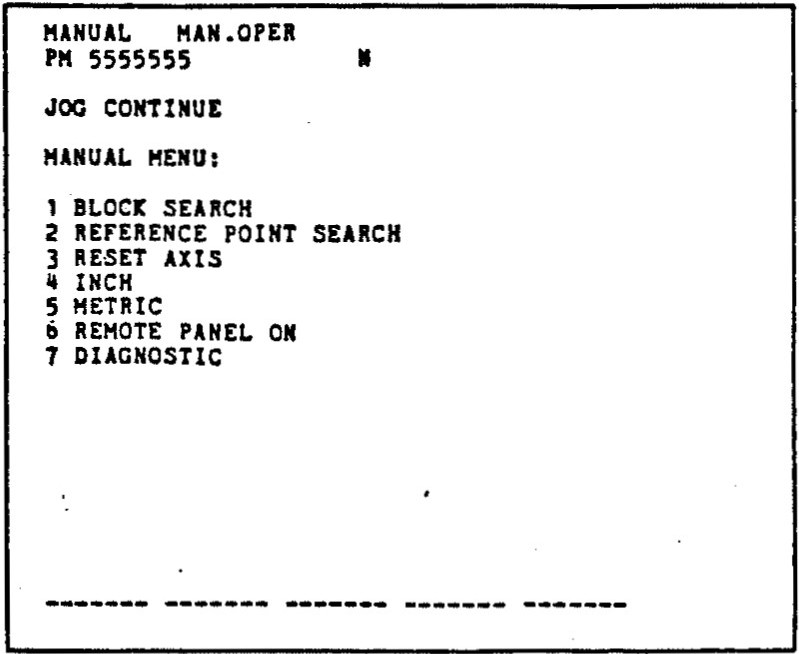
\includegraphics[width=0.6\textwidth]{manual_menu.jpg}
    \caption{Main Menu of Command Sub-Modes}
\end{figure}

\newpage

\begin{itemize}
    \item Press numeric key \textbf{3} to select \textbf{RESET AXIS}.
\end{itemize}

The following display appears on the screen:

\begin{figure}[h]
    \centering
    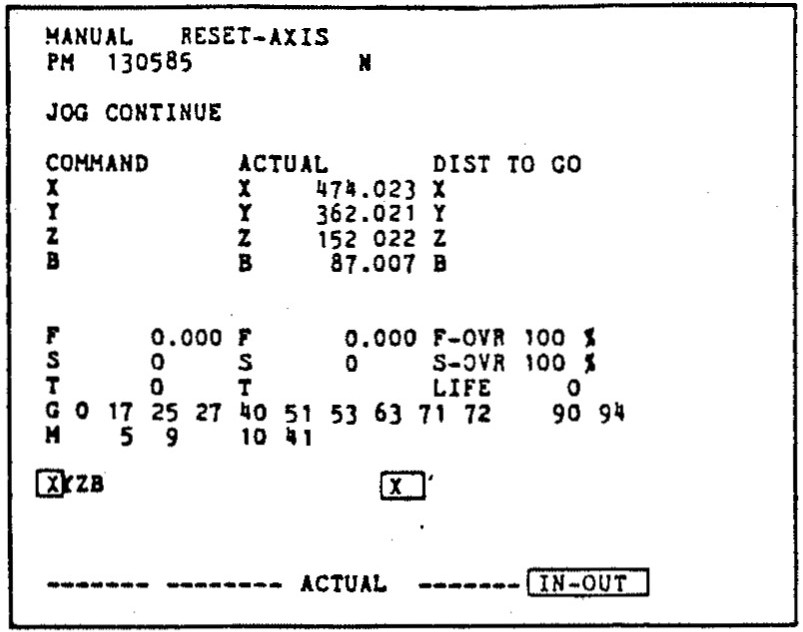
\includegraphics[width=0.7\textwidth]{reset_axis_screen.jpg}
    \caption{RESET AXIS Mode Display}
\end{figure}

\textbf{RESET AX} appears on \textbf{line 1} of the screen. The workpiece origin can now be set.

\subsubsection*{Assigning a Value of Zero to the Workpiece Origin}

The machine is positioned at the workpiece origin after referencing it step by step.

\begin{itemize}
    \iconitem {Move the cursor to the address letter of the desired axis using the \textbf{left} or \textbf{right} command buttons.}{left.jpg,right.jpg}
    \item Enter the value \textbf{0} using the keyboard.
    \iconitem {Press the \textbf{ENTER} button.}{enter.jpg}
    \vspace{.6cm}
    \iconitem {Press the \textbf{STORE} button.}{store.jpg}
\end{itemize}

\vspace{.5cm}

The value \textbf{0.000} is displayed on the screen for the selected axis under \textbf{ACTUAL}.

\begin{itemize}
    \iconitem {Press the \textbf{MANUAL} button to exit \textbf{RESET AXIS} mode.}{manual.jpg}
\end{itemize}

\vspace{1cm}

\newpage
\subsubsection*{Assigning Any Value to the Workpiece Origin}

The machine is \textbf{not positioned} at the workpiece origin after referencing it step by step.

For example, this occurs when the origin is referenced using a \textbf{measuring chuck, gauge blocks, or a sensor} (e.g., a Zentrikator).

\begin{itemize}
    \iconitem {Move the cursor to the address letter of the desired axis using the \textbf{left} or \textbf{right} command buttons.}{left.jpg,right.jpg}
    \item Enter the \textbf{offset value} relative to the workpiece origin, applying the \textbf{correct sign}, using the keyboard.
    
    \textit{(e.g., chuck radius + gauge block length).}
    \iconitem {Press the \textbf{ENTER} button.}{enter.jpg}
    \vspace{.6cm}
    \iconitem {Press the \textbf{STORE} button.}{store.jpg}
\end{itemize}

The \textbf{entered offset value} for the workpiece origin is displayed on the screen under \textbf{ACTUAL} for the selected axis.

\begin{itemize}
    \iconitem {Press the \textbf{MANUAL} button to exit \textbf{RESET AXIS} mode.}{manual.jpg}
\end{itemize}
\vspace{.5cm}
\notes

Setting the workpiece origin on the machine axes (\textbf{RESET AXIS}) automatically saves the \textbf{offset between the workpiece origin and the machine origin} in the system as an \textbf{origin shift}.

This memory of origin shifts is used in function \textbf{G52}.

\textbf{Activating stored origin shifts:} See Section 3.5.2.

\newpage
\section{Stored Origin Offsets (PROGRAM ZERO OFFSET)}

The workpiece origin offsets relative to the machine can be saved as \textbf{origin shifts} using functions \textbf{G52} and \textbf{G54 to G59} (\textbf{Z0 memory for origin shifts}).

\textbf{Origin shift entry and modification} is only possible in \textbf{MANUAL} mode.

\textbf{Writing and reading stored origin shifts:} See Section 8.2.5.

\procedure

\begin{itemize}
    \iconitem {Press the \textbf{MANUAL} button.}{manual.jpg}
    \vspace{.6cm}
    \iconitem {Press the \textbf{PROG.MEM} button.}{prog_mem.jpg}
    \vspace{.6cm}
    \iconitem {Press the \textbf{MENU} button.}{menu.jpg}
\end{itemize}
\vspace{.5cm}
The menu for programming machining parameters appears on the screen:

\begin{figure}[h]
    \centering
    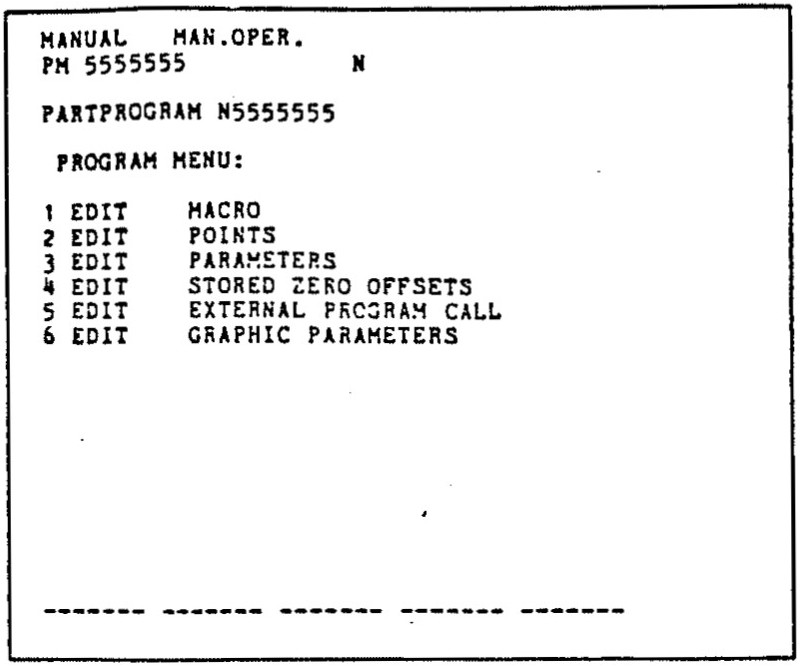
\includegraphics[width=0.7\textwidth]{program_menu.jpg}
    \caption{Program Menu Display}
\end{figure}

\begin{itemize}
    \item Press key \textbf{4} on the numeric keyboard to select \textbf{EDIT STORED ZERO OFFSET}.
\end{itemize}

\newpage

The list of \textbf{G functions} (\textbf{G51 to G59}) for stored origin offsets appears on the screen:

\begin{figure}[h]
    \centering
    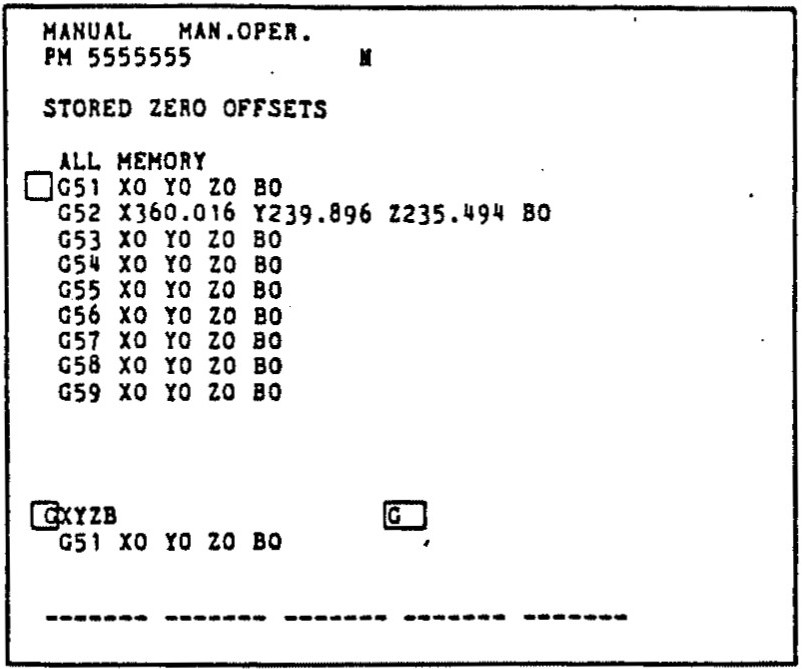
\includegraphics[width=0.7\textwidth]{stored_zero_offsets.jpg}
    \caption{Stored Zero Offsets Display}
\end{figure}

It is possible to enter or modify stored origin offsets in \textbf{EDIT STORED ZERO OFFSET} mode for functions \textbf{G54 to G59}.

The \textbf{G52} function also allows the entry or modification of an origin shift in this operating mode.

\textbf{G52} allows, without activating the \textbf{EDIT STORED ZERO OFFSET} mode, the automatic storage of the workpiece origin shift relative to the machine origin determined during the \textbf{RESET AXIS} operation (see Section 3.4.1).

The \textbf{G51} and \textbf{G53} functions in this list do not allow any entry or modification.

\textbf{G51 cancels G52.}

\textbf{G53 cancels G54 to G59.}

\notes

Stored origin offsets can be checked at any time during program execution.

Pressing the \textbf{PROG.MEM} and \textbf{MENU} buttons displays the menu for workpiece programming sub-modes on the screen. This menu also allows selecting the \textbf{DISPLAY STORED ZERO OFFSET} sub-mode (which displays stored origin offsets) instead of the \textbf{EDIT STORED ZERO OFFSET} mode.

\newpage

\subsection{Entering and Modifying Stored Origin Offsets}

Select the \textbf{EDIT STORED ZERO OFFSET} sub-mode (see Section 3.5), then:

\begin{itemize}
    \iconitem {Move the cursor to the line of the \textbf{G function} to be used for entering or modifying the origin offset. To do this, use the \textbf{up} and \textbf{down} command buttons.}{up.jpg,down.jpg}
    \iconitem {Move the cursor to the address letter of the selected axis using the \textbf{left} and \textbf{right} command buttons.}{left.jpg,right.jpg}
    \item Enter the \textbf{actual recorded value} of the workpiece origin for the selected axis (see Section 3.4.1).
    \iconitem {Press the \textbf{ENTER} button.}{enter.jpg}
    \vspace{.6cm}
    \iconitem {Press the \textbf{STORE} button after entering or modifying the actual origin values of the workpiece relative to other axes.}{store.jpg}
\end{itemize}

\vspace{.5cm}

Once the stored origin offsets have been entered into memory:

\begin{itemize}
    \iconitem {Press the \textbf{MANUAL} button.}{manual.jpg}
\end{itemize}

\vspace{.5cm}

\subsection{Activating a Stored Origin Offset}

A stored origin offset can be activated in \textbf{TEACH IN/MDI} mode by entering the corresponding \textbf{G function} and pressing the \textbf{START} button.

Executing the corresponding \textbf{G function} activates a stored origin offset \textbf{during the program}.

\subsection{Deleting Stored Origin Offsets}

Select the \textbf{EDIT STORED ZERO OFFSET} sub-mode (see Section 3.5), then:

\begin{itemize}
    \iconitem {Move the cursor to the line of the \textbf{G function} for which the origin offset should be deleted. Use the \textbf{up} and \textbf{down} command buttons.}{up.jpg,down.jpg}
    \iconitem {Press the \textbf{ENTER} button.}{enter.jpg}
    \vspace{.6cm}
    \item The selected \textbf{G function} is displayed on \textbf{line 14} of the screen with the remark \textbf{(CLEAR)}.
    \iconitem {Press the \textbf{STORE} button.}{store.jpg}
\end{itemize}

\vspace{.5cm}

Pressing the \textbf{STORE} button deletes the selected origin offset. The function corresponding to the deleted origin offset is now set to a value of \textbf{0} for each axis in the \textbf{G function list}.

If no further modifications need to be made to the stored origin offsets:

\begin{itemize}
    \iconitem {Press the \textbf{MANUAL} button.}{manual.jpg}
\end{itemize}

\newpage

\subsection{Deleting All Stored Origin Offsets}

Select the \textbf{EDIT STORED ZERO OFFSET} sub-mode (see Section 3.5), then:

\begin{itemize}
    \iconitem {Move the cursor to the \textbf{ALL MEMORY} line using the \textbf{up} and \textbf{down} command buttons.}{up.jpg,down.jpg}
\end{itemize}

\vspace{.5cm}

The \textbf{ALL MEMORY} signal is displayed on \textbf{line 21} of the screen.

\begin{itemize}
    \iconitem {Press the \textbf{ENTER} button.}{enter.jpg}
\end{itemize}

\vspace{.5cm}

The \textbf{ALL MEMORY} signal followed by \textbf{CLEAR} is displayed on \textbf{line 21} of the screen.

\begin{itemize}
    \iconitem {Press the \textbf{STORE} button.}{store.jpg}
\end{itemize}

\vspace{.5cm}

Pressing the \textbf{STORE} button deletes \textbf{all stored origin offsets} for the \textbf{G functions}.

If no further modifications need to be made to the stored origin offsets:

\begin{itemize}
    \iconitem {Press the \textbf{MANUAL} button.}{manual.jpg}
\end{itemize}
\vspace{.5cm}
\section{Manual Program Entry, Machine Stopped}

Part programs consist of either \textbf{main programs} or \textbf{subprograms}.

Main programs \textbf{PM} are stored in the memory for main programs, while subprograms \textbf{MM} are stored in the subprogram memory.

\textbf{Graphical interface and operator guidance:} See Section 3.9.

\procedure

\begin{itemize}
    \iconitem {Press the \textbf{MANUAL} button.}{manual.jpg}
    \vspace{.6cm}
    \iconitem {Press the \textbf{PROG.MEM} button (Program Memory).}{prog_mem.jpg}
\end{itemize}

\vspace{.5cm}

The following display appears on the screen:

\begin{figure}[h]
    \centering
    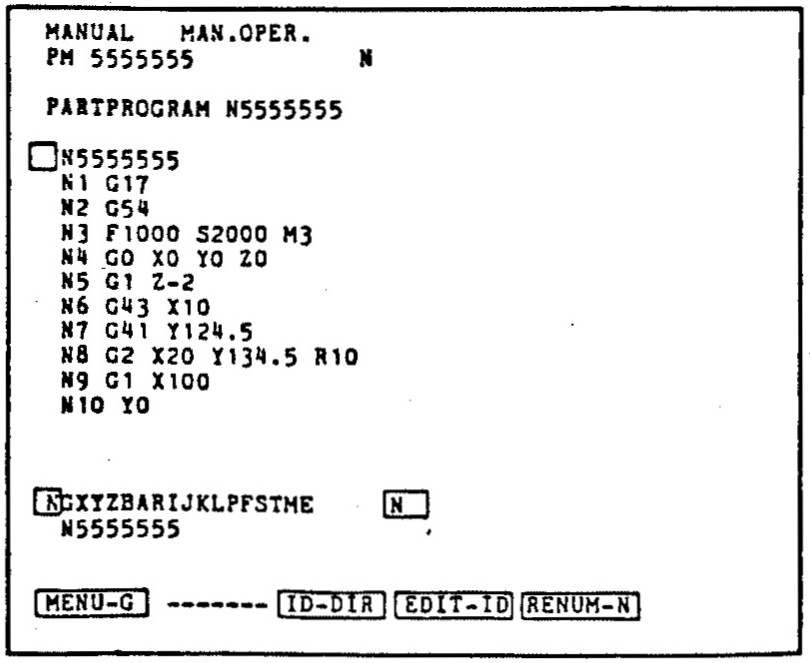
\includegraphics[width=0.6\textwidth]{program_memory_screen.jpg}
    \caption{Program Memory Display}
\end{figure}
\newpage

\begin{itemize}
    \iconitem {To now select the \textbf{subprogram memory}, press the sequence: \textbf{MENU, 1}.}{menu.jpg, one.jpg}
    \vspace{.5cm}
    \item Enter the number of the new program using the keyboard.
    \iconitem {Press the \textbf{ENTER} and \textbf{STORE} buttons.}{enter.jpg, store.jpg}
\end{itemize}

\vspace{.5cm}

Pressing the \textbf{STORE} button saves the new program number in memory. The number of the first block \textbf{N1} appears at \textbf{line 21} on the screen.

\begin{itemize}
    \iconitem {Move the cursor to the corresponding address letter using the \textbf{left} and \textbf{right} command buttons.}{left.jpg,right.jpg}
    \item Enter the numerical value using the keyboard.
    \iconitem {Press the \textbf{ENTER} button after each program word consisting of an address letter and a numerical value.}{enter.jpg}
    \vspace{.1cm}
    \iconitem {Press the \textbf{STORE} button once all program words for a block have been entered.}{store.jpg}
\end{itemize}

\vspace{.5cm}

The number of the second block \textbf{N2} then appears at \textbf{line 21} on the screen. Save the second block. The number of the third block \textbf{N3} then appears, and so on.

The last program blocks stored are displayed on the screen:

\begin{figure}[h]
    \centering
    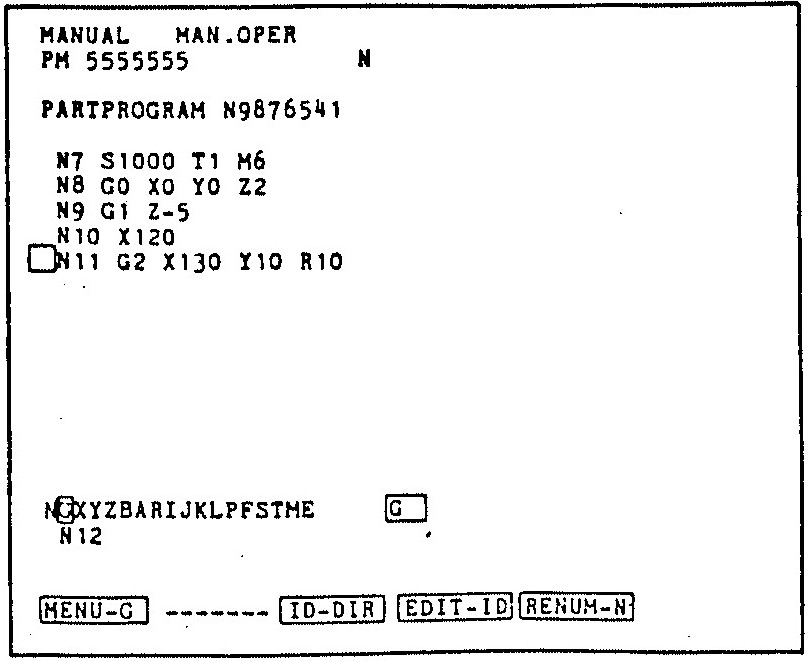
\includegraphics[width=0.7\textwidth]{stored_program_screen.jpg}
    \caption{Stored Program Blocks Display}
\end{figure}

\textbf{End of manual program entry:}

\begin{itemize}
    \iconitem {Press the \textbf{MANUAL} button.}{manual.jpg}
\end{itemize}

\newpage

\subsection{Entering Values Affecting Parameter E}

The parameters \textbf{E0 ... E255} simplify the programming process.

An \textbf{E parameter} must be defined before it can be used in a program.

A parameter is defined when it is assigned a numerical value, e.g.:

\begin{center}
    \fbox{\textbf{E3 = 123456}} \quad or \quad \fbox{\textbf{E4 = 789.123}}
\end{center}

Integer values and decimal values must have a maximum of \textbf{six digits}.

Decimal values can only contain \textbf{three digits after the decimal point}.

\procedure

The number of the program block to be entered is displayed on \textbf{line 21} of the screen.

\begin{itemize}
    \iconitem {Move the cursor to the address letter \textbf{E} using the \textbf{left} and \textbf{right} command buttons.}{left.jpg,right.jpg}
    \item Enter the \textbf{number} of the E parameter using the keyboard.
    \iconitem {Press the \textbf{EQUAL} button.}{equal.jpg}
    \vspace{.5cm}
    \item Enter the \textbf{value} of the E parameter using the keyboard.
    \iconitem {Press the \textbf{ENTER} button.}{enter.jpg}
    \vspace{.6cm}
    \iconitem {Press the \textbf{STORE} button.}{store.jpg}
\end{itemize}

\vspace{.5cm}

Pressing the \textbf{STORE} button saves the \textbf{E parameter} in memory. The defined parameter with its value can now be used in the program.

\newpage

\subsection{Calculation Operations with Parameter E}

The parameters \textbf{E0 ... E255} allow for calculations within the program.

Calculation operations can be performed using \textbf{two defined E parameters} (\textbf{Example 1}) or using a \textbf{defined E parameter and a numerical value} (\textbf{Example 2}).

\begin{center}
    \textbf{Example 1}: \fbox{\textbf{E8 = E4 - E3}}
    
    \textbf{Example 2}: \fbox{\textbf{E9 = E3 : 10.55}}
\end{center}

To the right of the \textbf{"="} sign, only previously defined \textbf{E parameters} may be used (see Section \textbf{3.6.1}).

\procedure

The number of the program block to be entered is displayed on \textbf{line 21} of the screen.

The parameters to the right of the equality sign (\textbf{E3} and \textbf{E4} in the given examples) must be \textbf{predefined}.

\begin{itemize}
    \iconitem {Move the cursor to the address letter \textbf{E} using the \textbf{left} and \textbf{right} command buttons.}{left.jpg,right.jpg}
    \item Enter the \textbf{number} of the E parameter using the keyboard.
    \iconitem {Press the \textbf{EQUAL} button.}{equal.jpg}
    \vspace{.6cm}
    \iconitem {Move the cursor back to the address letter \textbf{E} using the \textbf{left} and \textbf{right} command buttons.}{left.jpg,right.jpg}
    \item Enter the \textbf{number} of the E parameter using the keyboard.
    \iconitem {Press the \textbf{ENTER} button.}{enter.jpg}
\end{itemize}

The cursor is placed on the address letter \textbf{N} at \textbf{line 20} of the screen. \textbf{+N} is displayed on the right in the entry window.

The operation sign must now be entered.

\begin{itemize}
    \iconitem {Press the \textbf{OPER.} button as many times as necessary until the correct sign for the \textbf{desired operation} appears in the entry window.}{oper.jpg}
    \item Move the cursor:
    \begin{itemize}
        \item For \textbf{Example 1}, to the address letter \textbf{E}.
        \item For \textbf{Example 2}, to the \textbf{empty space} to the right of the address letter \textbf{E}.
    \end{itemize}
    \iconitem {Use the \textbf{left} and \textbf{right} command buttons to adjust.}{left.jpg,right.jpg}
    \vspace{.5cm}
    \item Enter the \textbf{number} of the E parameter (\textbf{Example 1}) or the \textbf{numerical value} (\textbf{Example 2}) via the keyboard.
    \iconitem {Press the \textbf{ENTER} button.}{enter.jpg}
\end{itemize}

The calculation operation that has just been entered is transferred to \textbf{line 21} of the screen.

\begin{itemize}
    \iconitem {Press the \textbf{STORE} button.}{store.jpg}
\end{itemize}

Pressing the \textbf{STORE} button saves the calculation operation. It is executed as soon as it is activated in the program and becomes effective for the next program.

\notes

The values of \textbf{E parameters} used in the machining program can be monitored at any time while the program is running (see \textbf{Section 7.8}).

\newpage

\section{Manual Entry of Programs During Program Execution}

The \textbf{TEACH IN}, \textbf{SINGLE}, and \textbf{AUTO} modes allow a new machining program to be entered into the memory of main programs or sub-programs.

\procedure

\begin{itemize}
    \iconitem {Press the \textbf{PROG.MEM} button (selection of main program memory).}{prog_mem.jpg}
    \vspace{.5cm}
    \item Enter the number of the new program via the keyboard.
    \iconitem {Press the \textbf{ENTER} and \textbf{STORE} buttons.}{enter.jpg,store.jpg}
\end{itemize}

\vspace{.5cm}

Pressing the \textbf{STORE} button saves the program number. The screen displays the number of the first program block \textbf{N1} on \textbf{line 21}.

\begin{itemize}
    \item \textbf{Continuation of program entry:} See \textbf{Section 3.6}.
\end{itemize}

\vspace{.5cm}

Once the program has been completely entered:

\begin{itemize}
    \iconitem {Press the \textbf{TEACH IN}, \textbf{SINGLE}, or \textbf{AUTO} button according to the signal displayed on \textbf{line 1} of the screen (\textbf{TEACH IN}, \textbf{SINGLE}, or \textbf{AUTO}).}{teach_in.jpg,single.jpg,auto.jpg}
\end{itemize}

\vspace{.5cm}

Pressing the corresponding button causes the display of the selected operating mode to appear on the screen.

\newpage

\section{Maskable Blocks}

Maskable blocks are program blocks that can be \textbf{masked} in the program when necessary. In this case, they are skipped during program execution.

Maskable blocks must be identified as such by placing a forward slash \textbf{/} before the block number \textbf{N}.

Maskable blocks can be used in both main programs and sub-programs.

\subsection{Programming Maskable Blocks}

The number of the program block to be entered is displayed on \textbf{line 21} of the screen.

\begin{itemize}
    \iconitem{ Move the cursor to the address letter \textbf{N} using the \textbf{left} and \textbf{right} command buttons.}{left.jpg, right.jpg}
    \vspace{.1cm}
    \iconitem {Press the \textbf{sign change} button.}{sign_change.jpg}
\end{itemize}
\vspace{.5cm}
A forward slash \textbf{/} precedes the block number on \textbf{line 20} of the screen: \textbf{/N}.

\begin{itemize}
    \item Enter the block number via the keyboard.
    \iconitem {Press the \textbf{ENTER} button.}{enter.jpg}
    \vspace{.5cm}
    \item \textbf{Continuation of the procedure:} See \textbf{Section 3.6}.
\end{itemize}

\vspace{.5cm}

notes

It is possible to convert a maskable block into a non-maskable block if needed (i.e., not skipped). In this case, the program number must be re-entered after selecting the maskable block \textbf{/N}, and the entire block must be stored again.

A block that cannot be skipped can be converted into a maskable block when necessary. To do so, select block \textbf{N}, press the \textbf{sign change} button, and store the entire block.

\textbf{Skipping Maskable Blocks:} See \textbf{Section 7.2}.

\newpage

\section{Graphical Interface and Operator Guidance}

The operator guidance procedure can be selected for data entry in the following operating modes: \textbf{TEACH-IN/MDI, TEACH-IN/PLAYBACK, "MANUAL PART PROGRAM"} and \textbf{MANUAL MACRO}.

Operator guidance allows data input through a structured address-letter line with a concise description of the letter-address. The most important functions can also be represented more graphically using \textbf{support graphics}.

\procedure

\begin{itemize}
    \iconitem {Press the \textbf{MANUAL} button.}{manual.jpg}
    \vspace{.6cm}
    \iconitem {Press the \textbf{TEACH-IN} button or the \textbf{PROG.MEM} button.}{teach_in.jpg, prog_mem.jpg}
\end{itemize}

\vspace{.5cm}

The mode \textbf{TEACH-IN/MDI} or \textbf{MANUAL PART PROGRAM} is selected.

\begin{itemize}
    \iconitem {Press the \textbf{MENU} button, then the \textbf{1} key on the numeric keyboard.}{menu.jpg, one.jpg}
\end{itemize}

The mode \textbf{TEACH-IN PLAYBACK} or \textbf{MANUAL MACRO} is selected.

\textbf{For the following operating modes:}

\begin{itemize}
    \item \textbf{TEACH-IN MDI}
    \item \textbf{TEACH-IN PLAYBACK}
    \item \textbf{MANUAL PART PROGRAM}
\end{itemize}

After saving the program number, this also applies to the \textbf{MANUAL MACRO} mode.

The display of \textbf{F1 MENU-G} for the function button appears in an inverted format on \textbf{line 24} of the screen.

\underline{Procedure for the MANUAL MACRO mode}

\begin{itemize}
    \item Enter the program number for the new program using the numeric keyboard.
    \iconitem {Press the \textbf{ENTER} and \textbf{STORE} buttons.}{enter.jpg, store.jpg}
\end{itemize}

\subsubsection*{Selection of the "Operator Guidance" Procedure}

\begin{itemize}
    \iconitem {Press the \textbf{F1} button.}{f1.jpg}
\end{itemize}

Pressing the \textbf{F1} button activates the operator guidance procedure.

The display of the shortened letter-address line appears on \textbf{line 20} of the screen, and the description of letter-addresses appears on \textbf{line 19}.

\textbf{FREE-G} for function button \textbf{F1} and \textbf{PICTURE} for function button \textbf{F2} are displayed in an inverted format on \textbf{line 24}. For the most important \textbf{G functions}, it is possible to select the support graphics.

\subsubsection*{Selection of the "Support Graphics" Procedure}

\begin{itemize}
    \iconitem {Press the \textbf{F2} button.}{f2.jpg}
\end{itemize}

Pressing the \textbf{F2} button connects the support graphics procedure. For certain \textbf{G functions}, \textbf{PICTURE} remains displayed in an inverted format on \textbf{line 24} for function button \textbf{F2}.

The images for the support graphics can be changed by pressing the \textbf{F2} button multiple times.

\subsubsection*{Cancellation of the "Operator Guidance" or "Support Graphics and Operator Guidance" Procedure}

\begin{itemize}
    \iconitem {Press the \textbf{F1} button.}{f1.jpg}
\end{itemize}

After pressing the \textbf{F1} button, variable programming of \textbf{G functions} is activated.

\textbf{MENU-G} for function button \textbf{F1} is displayed in an inverted format on \textbf{line 24} of the screen.

\notes

In \textbf{SINGLE} and \textbf{AUTO} operating modes, the operator guidance procedures and support graphics can also be used for controlling \textbf{PART PROGRAM} or \textbf{MACRO}.